\chapter{Trabalho, energia e energia potencial}\label{ch:b1:work-and-energy}

Um ciclista para de pedalar no alto de um morro e chega embaixo
com uma velocidade que depende do desnível, não do traçado da estrada. Um
saltador de bungee jump cai sessenta metros e para, por um instante, exatamente
onde a tração da corda consumiu toda a velocidade que a queda havia dado. Um
átomo de hidrogênio ligado a um átomo de cloro vibra num poço cuja profundidade
é a energia necessária para despedaçar a molécula. Em cada caso um
único número é trocado entre formas --- movimento, altura, alongamento,
ligação --- e, somado, não muda. Este capítulo constrói essa
contabilidade a partir da segunda lei de Newton: \omterm{def:b1:work-and-energy:work}{trabalho} e potência, o teorema
da \omterm{thm:b1:work-and-energy:ke}{energia cinética}, \omterm{def:b1:work-and-energy:conservative}{energias potenciais} para as forças que as admitem e
a \omterm{thm:b1:work-and-energy:em}{conservação da energia mecânica}, que transforma muitos problemas de dinâmica
numa álgebra de uma linha e explica, pela forma de um \omterm{def:b1:work-and-energy:turning}{poço de
potencial}, quais posições são estáveis.

\begin{omfigure}
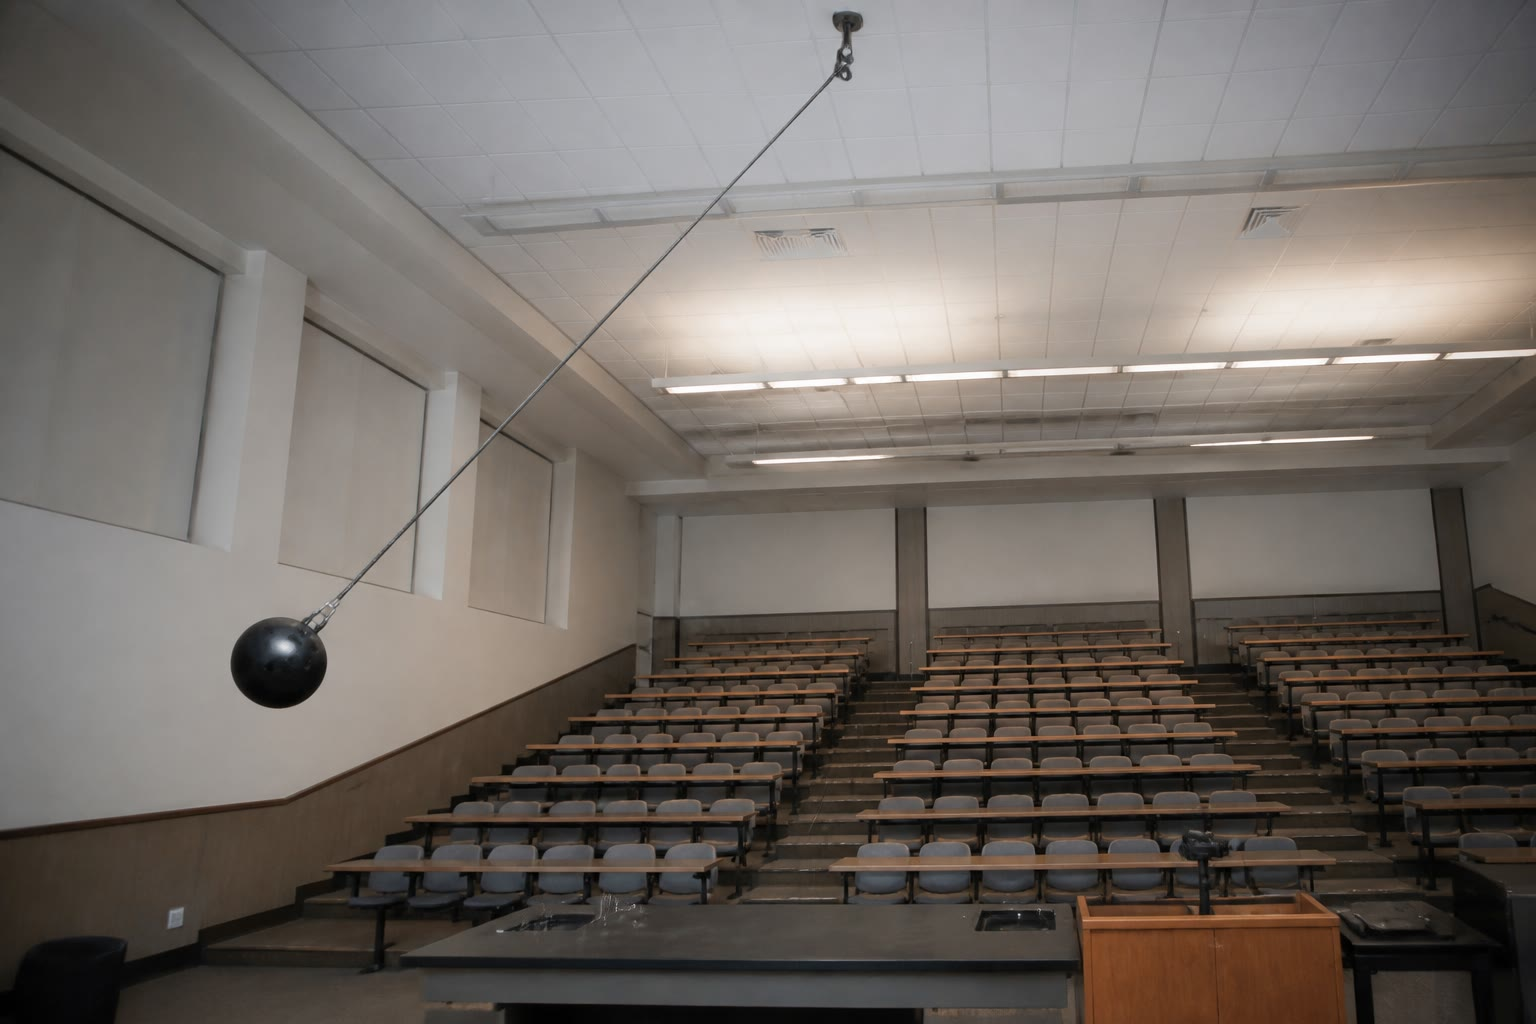
\includegraphics[width=0.58\linewidth]{images/book3/ai/b3-13-lecture-hall-pendulum.jpg}

{\small O pêndulo do professor: solta junto ao nariz, a bola de boliche volta ao nariz e não passa dele --- a \omterm{thm:b1:work-and-energy:em}{energia mecânica} se conserva, e nunca é excedida.}
\end{omfigure}

\section{Potência e trabalho}

\begin{definition}[Potência e trabalho de uma força]\label{def:b1:work-and-energy:work}
\index{potência (de uma força)}\index{trabalho}
A \emph{potência} de uma força $\vect F$ que age sobre um ponto que se move com
velocidade $\vect v$ é
\[
\mathcal P = \vect F\cdot\vect v \qquad (\text{watts}),
\]
e o seu \emph{trabalho} entre os instantes $t_1$ e $t_2$ (posições $A$ e $B$)
é a potência acumulada,
\[
W_{A\to B} = \int_{t_1}^{t_2}\vect F\cdot\vect v\,\dd t
= \int_A^B \vect F\cdot\dd\vect\ell \qquad (\text{joules}),
\]
a soma dos \emph{trabalhos elementares} $\delta W = \vect F\cdot\dd\vect\ell$
ao longo dos deslocamentos elementares $\dd\vect\ell = \vect v\,\dd t$ da
\omterm{def:b1:point-kinematics:frame}{trajetória}. O trabalho é positivo se a força empurra no sentido do movimento
(\emph{motor}), negativo se contra ele (\emph{resistente}) e nulo se
perpendicular.
\end{definition}

\begin{proposition}[Trabalhos que se encontram]\label{prop:b1:work-and-energy:works}
\begin{itemize}
  \item Força constante: $W_{A\to B} = \vect F\cdot\vect{AB}$, qualquer que seja o
        caminho. Peso: $W = mg(z_A - z_B)$, com $z$ contado para cima.
  \item Mola de constante elástica $k$, do alongamento $x_A$ a $x_B$:
        $W = \tfrac12 k(x_A^2 - x_B^2)$.
  \item \omterm{prop:b1:newton-dynamics:friction}{Reação normal} de uma superfície fixa, tensão de um fio sobre um corpo
        que se move perpendicularmente a ele: $W = 0$ (força $\perp$ deslocamento).
  \item Atrito cinético e arrasto: $W < 0$ sempre (a força se opõe ao
        movimento relativo), e depende do comprimento do caminho.
\end{itemize}
\end{proposition}

\begin{proof}
Com $\vect F$ constante: $\int\vect F\cdot\dd\vect\ell = \vect F\cdot\int\dd\vect\ell
= \vect F\cdot\vect{AB}$; com $\vect F = -mg\vect e_z$, $\vect F\cdot\vect{AB}
= -mg(z_B - z_A)$. Mola: $\vect F\cdot\dd\vect\ell = -kx\,\dd x$, e
$\int_{x_A}^{x_B}-kx\,\dd x = \tfrac12 k(x_A^2 - x_B^2)$. Atrito: $\vect T
= -\mu N\vect v/v$, logo $\vect T\cdot\vect v = -\mu Nv < 0$.
\end{proof}

\begin{omfigure}
\begin{tikzpicture}[font=\small, x=1cm, y=1cm]
  \draw[omDef, thick, domain=0:6, samples=60] plot (\x, {0.35*\x + 0.9*sin(deg(0.7*\x))});
  \fill (0,0) circle (1.4pt) node[below] {$A$};
  \fill (6,{2.1+0.9*sin(deg(4.2))}) circle (1.4pt) node[right] {$B$};
  % point at x=2.4: y = 0.84+0.9*sin(96.3deg)=0.84+0.894=1.734 ; slope 0.35+0.63cos(96.3)=0.35-0.069=0.28
  \coordinate (M) at (2.4,1.734);
  \fill[omThm] (M) circle (1.6pt); \node[above left] at (M) {$M$};
  \draw[-Stealth, omThm, very thick] (M) -- ++(1.1,0.31) node[right] {$\dd\vect\ell$};
  \draw[-Stealth, omProp, very thick] (M) -- ++(1.4,-0.9) node[below right] {$\vect F$};
  \draw ($(M)+(0.55,0.15)$) arc (15.6:-32.7:0.57); \node at ($(M)+(0.85,-0.12)$) {$\alpha$};
  \node[omExo, font=\footnotesize] at (3.6,3.4) {$\delta W = \vect F\cdot\dd\vect\ell = F\,\dd\ell\cos\alpha$};
\end{tikzpicture}

{\small O \omterm{def:b1:work-and-energy:work}{trabalho} elementar de uma força ao longo de um pequeno deslocamento do
seu ponto de aplicação: só a componente de $\vect F$ ao longo do
movimento realiza \omterm{def:b1:work-and-energy:work}{trabalho}. Somado ao longo do caminho de $A$ a $B$, ele dá
$W_{A\to B}$.}
\end{omfigure}

\section{O teorema da energia cinética}

\begin{theorem}[Teoremas da energia cinética e da potência]\label{thm:b1:work-and-energy:ke}
\index{energia cinética}\index{teorema da energia cinética}
Num \omterm{thm:b1:newton-dynamics:laws}{referencial inercial}, a \emph{\omterm{thm:b1:work-and-energy:ke}{energia cinética}} $E_k = \tfrac12 mv^2$ de
um \omterm{def:b1:point-kinematics:frame}{ponto material} obedece a
\[
\frac{\dd E_k}{\dd t} = \sum\mathcal P_i = \Big(\sum\vect F_i\Big)\cdot\vect v,
\qquad
E_k(B) - E_k(A) = \sum_i W_{i,A\to B}:
\]
a variação da \omterm{thm:b1:work-and-energy:ke}{energia cinética} entre duas posições é igual ao \omterm{def:b1:work-and-energy:work}{trabalho} total
de todas as forças aplicadas ao longo do caminho.
\end{theorem}

\begin{proof}
Multiplique escalarmente a segunda lei de Newton por $\vect v$: $m\vect a\cdot\vect v =
\tfrac{\dd}{\dd t}(\tfrac12 m\vect v\cdot\vect v) = \dd E_k/\dd t$, enquanto
$(\sum\vect F_i)\cdot\vect v = \sum\mathcal P_i$. Integre no tempo.
\end{proof}

\begin{example}[Distância de frenagem]\label{ex:b1:work-and-energy:braking}
Um carro de \qty{1000}{kg} a \qty{100}{km/h} ($E_k = \qty{386}{kJ}$) freado por
uma força constante de \qty{7.0}{kN} para depois de $d = E_k/F = \qty{55}{m}$:
a distância cresce com o \emph{quadrado} da velocidade. Como a
força máxima de frenagem vale $\mu_smg$ (\cref{ch:b1:newton-dynamics}), a
menor distância de parada é $v^2/2\mu_sg$, qualquer que seja a massa do carro ---
e ela dobra numa pista molhada, onde $\mu_s$ cai à metade.
\end{example}

\section{Forças conservativas e energia potencial}

\begin{definition}[Força conservativa; energia potencial]\label{def:b1:work-and-energy:conservative}
\index{força conservativa}\index{energia potencial}
Uma força é \emph{conservativa} se o seu \omterm{def:b1:work-and-energy:work}{trabalho} entre dois pontos não
depende do caminho seguido. De modo equivalente, existe uma função da
posição, a \emph{energia potencial} $E_p$, tal que
\[
W_{A\to B} = E_p(A) - E_p(B) = -\Delta E_p ,
\qquad \delta W = -\dd E_p ,
\]
sendo $E_p$ definida a menos de uma constante aditiva (uma escolha de origem).
\end{definition}

\begin{proposition}[A força a partir da energia potencial]\label{prop:b1:work-and-energy:gradient}
\index{gradiente}
Uma \omterm{def:b1:work-and-energy:conservative}{força conservativa} deriva da sua \omterm{def:b1:work-and-energy:conservative}{energia potencial}:
\[
\vect F = -\overrightarrow{\operatorname{grad}}\,E_p
= -\frac{\partial E_p}{\partial x}\,\vect e_x
- \frac{\partial E_p}{\partial y}\,\vect e_y
- \frac{\partial E_p}{\partial z}\,\vect e_z ,
\]
e em uma dimensão $F_x = -\dd E_p/\dd x$: a força aponta no sentido em que a
\omterm{def:b1:work-and-energy:conservative}{energia potencial} decresce, ``ladeira abaixo'' no gráfico de $E_p$.
\end{proposition}

\begin{proof}
$\delta W = F_x\dd x + F_y\dd y + F_z\dd z = -\dd E_p = -(\partial_xE_p\,\dd x
+ \partial_yE_p\,\dd y + \partial_zE_p\,\dd z)$ para todo deslocamento:
identifique os coeficientes (a diferencial de uma função de várias
variáveis, do curso de matemática).
\end{proof}

\begin{proposition}[As energias potenciais usuais]\label{prop:b1:work-and-energy:eps}
\index{energia potencial!gravitacional}\index{energia potencial!elástica}
\begin{itemize}
  \item Peso: $E_p = mgz + \text{const}$ (com $z$ para cima).
  \item Mola: $E_p = \tfrac12 k(\ell - \ell_0)^2 + \text{const}$.
  \item Gravitação newtoniana de uma massa $M$: $E_p = -GMm/r + \text{const}$,
        com a constante escolhida em geral para que $E_p \to 0$ no infinito.
  \item Força eletrostática sobre uma carga $q$ num potencial $V$:
        $E_p = qV$ (\cref{ch:b1:potential-capacitors}).
\end{itemize}
O atrito cinético e o arrasto fluido \emph{não} são conservativos (o seu \omterm{def:b1:work-and-energy:work}{trabalho}
depende do caminho e é sempre negativo).
\end{proposition}

\begin{proof}
Cada uma se lê nos \omterm{def:b1:work-and-energy:work}{trabalhos} da \cref{prop:b1:work-and-energy:works}:
$W = -\Delta E_p$. Para a gravitação, $\vect F = -GMm/r^2\,\vect e_r$ e
$\delta W = -GMm\,\dd r/r^2 = -\dd(-GMm/r)$.
\end{proof}

\section{Energia mecânica}

\begin{theorem}[Energia mecânica]\label{thm:b1:work-and-energy:em}
\index{energia mecânica}\index{conservação da energia mecânica}
Seja $E_m = E_k + E_p$ a \emph{\omterm{thm:b1:work-and-energy:em}{energia mecânica}}, em que $E_p$ é a
soma das \omterm{def:b1:work-and-energy:conservative}{energias potenciais} das \omterm{def:b1:work-and-energy:conservative}{forças conservativas}. Então
\[
\Delta E_m = W_{\text{nc}} ,
\]
o \omterm{def:b1:work-and-energy:work}{trabalho} total das forças não conservativas. Se estas não realizam \omterm{def:b1:work-and-energy:work}{trabalho}
(sem atrito, ou com forças de vínculo perpendiculares ao movimento), $E_m$
se \emph{conserva}: o movimento é \emph{conservativo}.
\end{theorem}

\begin{proof}
$\Delta E_k = W_{\text{c}} + W_{\text{nc}} = -\Delta E_p + W_{\text{nc}}$.
\end{proof}

\begin{method}[Usando a energia]\label{met:b1:work-and-energy:method}
Quando um problema pede uma \emph{velocidade numa posição} (não um tempo, nem uma
força), tente a energia primeiro:
\begin{enumerate}
  \item liste as forças; veja quais realizam \omterm{def:b1:work-and-energy:work}{trabalho} e quais são conservativas;
  \item escreva $E_m$ nas duas posições, com uma origem clara para $E_p$;
  \item iguale-as (somando $W_{\text{nc}}$ se houver atrito) e resolva
        para a velocidade ou a posição desconhecida.
\end{enumerate}
A energia nunca dá o tempo nem as forças de vínculo; para essas, volte
à lei de Newton --- muitas vezes com a velocidade que a energia acabou de fornecer.
\end{method}

\begin{example}[A lei da velocidade do loop]\label{ex:b1:work-and-energy:loop}
No loop sem atrito do \cref{pb:b1:point-kinematics:1}, a reação da pista
é normal ao movimento e não realiza \omterm{def:b1:work-and-energy:work}{trabalho}: $E_m$ se conserva.
Com $z = R(1 - \cos\theta)$ acima do ponto mais baixo, $\tfrac12 mv^2 + mgR(1 -
\cos\theta) = \tfrac12 mv_0^2$: a lei da velocidade $v^2 = v_0^2 - 2gR(1 -
\cos\theta)$ ali usada, agora deduzida em uma linha. A velocidade mínima de
entrada $\sqrt{5gR}$ decorre então da condição no alto,
$v^2 \geq gR$, do \cref{ex:b1:newton-dynamics:circles}.
\end{example}

\begin{example}[Energia perdida no atrito]\label{ex:b1:work-and-energy:friction}
Um bloco desce uma rampa de ângulo $\alpha$ e altura $h$ com
atrito cinético $\mu_d$: $W_{\text{nc}} = -\mu_dmg\cos\alpha \times
h/\sin\alpha = -\mu_dmgh\cot\alpha$, logo $\tfrac12 mv^2 = mgh(1 - \mu_d\cot\alpha)$.
Para $h = \qty{2.0}{m}$, $\alpha = 30^\circ$, $\mu_d = 0.20$: $v =
\qty{5.1}{m/s}$ em vez de $\qty{6.3}{m/s}$; um terço da \omterm{def:b1:work-and-energy:conservative}{energia
potencial} virou calor.
\end{example}

\section{Equilíbrio, estabilidade e retratos de fase}

\begin{proposition}[Equilíbrio e estabilidade em uma dimensão]\label{prop:b1:work-and-energy:stability}
\index{equilíbrio!estável, instável}\index{pequenas oscilações}
Um \omterm{def:b1:point-kinematics:frame}{ponto material} que se move sobre um eixo sob uma \omterm{def:b1:work-and-energy:conservative}{força conservativa} de \omterm{def:b1:work-and-energy:conservative}{energia
potencial} $E_p(x)$:
\begin{itemize}
  \item está em \emph{equilíbrio} em $x_0$ se e só se $F(x_0) = -E_p'(x_0) = 0$:
        nos extremos de $E_p$;
  \item o equilíbrio é \emph{estável} se $E_p$ tem ali um mínimo local
        ($E_p''(x_0) > 0$): um pequeno deslocamento produz uma
        força restauradora; é \emph{instável} num máximo;
  \item perto de um equilíbrio estável, os pequenos movimentos são harmônicos, com
        \[
        \omega_0^2 = \frac{E_p''(x_0)}{m} .
        \]
\end{itemize}
\end{proposition}

\begin{proof}
Fórmula de Taylor (curso de matemática): $E_p(x) \approx E_p(x_0) +
\tfrac12 E_p''(x_0)(x - x_0)^2$, logo $F \approx -E_p''(x_0)(x - x_0)$ e
$m\ddot x = -E_p''(x_0)(x - x_0)$ --- uma mola de constante elástica $E_p''(x_0)$.
Para $E_p'' < 0$ a ``constante elástica'' é negativa: afastamento exponencial.
\end{proof}

\begin{omfigure}
\begin{tikzpicture}
\begin{axis}[omaxis, axis x line=bottom, axis y line=left, width=10.5cm, height=5.8cm, xlabel={$x$}, ylabel={$E_p$},
    xlabel style={at={(axis description cs:0.5,-0.06)}, anchor=north},
    xmin=-2.3, xmax=2.5, ymin=-1.5, ymax=1.6, xtick={-1,1}, xticklabels={$-a$,$a$}, ytick=\empty]
  \addplot[omDef, thick, domain=-2.15:2.15, samples=200] {x^4 - 2*x^2 + 0.3*x};
  \addplot[omThm, dashed, domain=-2.3:2.5, samples=2] {-0.45};
  \addplot[omExo, dashed, domain=-2.3:2.5, samples=2] {0.9};
  \node[omThm, font=\footnotesize, anchor=east] at (axis cs:2.45,-0.3) {$E_1$};
  \node[omExo, font=\footnotesize, anchor=east] at (axis cs:2.45,1.05) {$E_2$};
  \node[font=\footnotesize, below] at (axis cs:-1.08,-0.7) {estável};
  \node[font=\footnotesize, above] at (axis cs:0.08,0.08) {instável};
  \node[font=\footnotesize, below] at (axis cs:0.97,-1.1) {estável};
  \draw[Stealth-Stealth, omThm] (axis cs:-1.56,-0.45) -- (axis cs:-0.47,-0.45);
  \draw[Stealth-Stealth, omThm] (axis cs:0.42,-0.45) -- (axis cs:1.48,-0.45);
\end{axis}
\end{tikzpicture}

{\small Uma paisagem de potencial unidimensional: os mínimos são equilíbrios
estáveis, e o máximo é um equilíbrio instável. Um \omterm{def:b1:point-kinematics:frame}{ponto material} de energia $E_1$
abaixo da barreira fica preso num poço entre dois \emph{\omterm{def:b1:work-and-energy:turning}{pontos de
retorno}} (onde $E_p = E_1$, setas) e oscila; com $E_2$ acima
da barreira ele passa livremente de um poço ao outro.}
\end{omfigure}

\begin{definition}[Pontos de retorno; movimento ligado e livre]\label{def:b1:work-and-energy:turning}
\index{ponto de retorno}\index{movimento ligado}\index{poço de potencial}\index{barreira de potencial}
Para um movimento unidimensional conservativo de energia $E_m$, o \omterm{def:b1:point-kinematics:frame}{ponto material}
só pode estar onde $E_p(x) \leq E_m$ (pois $E_k \geq 0$); os pontos em que
$E_p = E_m$ são \emph{pontos de retorno}, em que a velocidade se anula e
se inverte. Preso entre dois pontos de retorno num \emph{poço de potencial},
o movimento é \emph{ligado} e periódico; se puder alcançar o infinito, ele é
\emph{livre}; uma \emph{barreira de potencial} mais alta que $E_m$ não pode ser
atravessada.
\end{definition}

\begin{definition}[Retrato de fase]\label{def:b1:work-and-energy:phase}
\index{retrato de fase}
O \emph{retrato de fase} de um movimento unidimensional é a família de
curvas traçadas pelo ponto $(x, \dot x)$ no \emph{plano de fase}. Para
um sistema conservativo cada curva é uma linha de nível $\tfrac12 m\dot x^2 +
E_p(x) = E_m$: curvas fechadas em torno dos equilíbrios estáveis (oscilações),
curvas abertas para o movimento livre e, passando pelos equilíbrios instáveis, as
\emph{separatrizes} que dividem os dois casos. As curvas são percorridas no sentido horário
($\dot x > 0$ significa $x$ crescente) e nunca se cruzam.
\end{definition}

\begin{omfigure}
\begin{tikzpicture}
\begin{axis}[omaxis, width=11cm, height=6.2cm, xlabel={$\theta$}, ylabel={$\dot\theta/\omega_0$},
    xmin=-7.2, xmax=7.2, ymin=-2.6, ymax=2.6, xtick={-6.283,-3.1416,0,3.1416,6.283},
    xticklabels={$-2\pi$,$-\pi$,$0$,$\pi$,$2\pi$}, ytick={-2,2}]
  % closed curves: thetadot^2 = 2(e - (1 - cos theta)) with e<2 ; thetadot = ±sqrt(2(e-1+cos))
  \foreach \e/\tm in {0.3/0.795, 1.0/1.5708, 1.7/2.346} {
    \foreach \sh in {0, 6.2832, -6.2832} {
      \addplot[omDef, thick, domain=-\tm:\tm, samples=200] ({x+\sh},{sqrt(max(0,2*(\e-1+cos(deg(x)))))});
      \addplot[omDef, thick, domain=-\tm:\tm, samples=200] ({x+\sh},{-sqrt(max(0,2*(\e-1+cos(deg(x)))))});
    }
  }
  % separatrix e=2
  \addplot[omThm, thick, domain=-7.2:7.2, samples=400] {sqrt(2*(1+cos(deg(x))))};
  \addplot[omThm, thick, domain=-7.2:7.2, samples=400] {-sqrt(2*(1+cos(deg(x))))};
  % rotations e=2.5, 3.2
  \foreach \e in {2.6,3.4} {
    \addplot[omProp, thick, domain=-7.2:7.2, samples=300] {sqrt(2*(\e-1+cos(deg(x))))};
    \addplot[omProp, thick, domain=-7.2:7.2, samples=300] {-sqrt(2*(\e-1+cos(deg(x))))};
  }
  \fill (axis cs:0,0) circle (1.5pt); \fill (axis cs:3.1416,0) circle (1.5pt); \fill (axis cs:-3.1416,0) circle (1.5pt);
\end{axis}
\end{tikzpicture}

{\small \omterm{def:b1:work-and-energy:phase}{Retrato de fase} do \omterm{ex:b1:newton-dynamics:pendulum}{pêndulo simples}, $\tfrac12\dot\theta^2 +
\omega_0^2(1 - \cos\theta) = \text{const}$. Curvas fechadas (azuis): oscilações
em torno do equilíbrio estável $\theta = 0$; curvas abertas (laranja): rotações
completas; entre elas a separatriz (vermelha) pelos equilíbrios
instáveis $\theta = \pm\pi$, o movimento que apenas alcança o topo.}
\end{omfigure}

\begin{example}[A paisagem do pêndulo]\label{ex:b1:work-and-energy:pendulum}
$E_p = -mg\ell\cos\theta$: mínimo em $\theta = 0$, $E_p'' = mg\ell$, logo
$\omega_0^2 = g\ell/(m\ell^2) = g/\ell$ --- o resultado das \omterm{prop:b1:work-and-energy:stability}{pequenas oscilações} do
\cref{ex:b1:newton-dynamics:pendulum}, lido na curvatura do poço;
máximo em $\theta = \pi$, o pêndulo invertido, instável. Energia
$E_m < mg\ell$: oscilação entre $\pm\theta_{\max}$; $E_m > mg\ell$: ele
passa por cima e gira; $E_m = mg\ell$: a separatriz, uma
aproximação infinitamente lenta ao topo.
\end{example}

\section{Exercícios}

\begin{exercise}[$\star$]\label{exo:b1:work-and-energy:1}
Uma caixa de \qty{20}{kg} é erguida \qty{3.0}{m} com velocidade constante em
\qty{5.0}{s}. \omterm{def:b1:work-and-energy:work}{Trabalho} da força que ergue, do peso, e potência
fornecida. A mesma caixa empurrada \qty{3.0}{m} por um piso com
$\mu_d = 0.30$: \omterm{def:b1:work-and-energy:work}{trabalho} do atrito.
\end{exercise}

\begin{exercise}[$\star$]\label{exo:b1:work-and-energy:2}
\omterm{thm:b1:work-and-energy:ke}{Energia cinética} de um carro de \qty{1000}{kg} a \qty{100}{km/h}; distância de
parada com uma força de frenagem constante de \qty{7.0}{kN}; o que acontece com
a distância se a velocidade dobrar?
\end{exercise}

\begin{exercise}[$\star$]\label{exo:b1:work-and-energy:3}
Uma mola de constante elástica \qty{500}{N/m} é comprimida \qty{10}{cm} e
solta contra uma bola de \qty{50}{g} numa pista horizontal sem atrito.
Energia armazenada; velocidade da bola.
\end{exercise}

\begin{exercise}[$\star$]\label{exo:b1:work-and-energy:4}
Um pêndulo de comprimento \qty{1.0}{m} é solto do repouso a $60^\circ$:
velocidade embaixo pela energia; depois, com a lei de Newton, a tensão
ali (em unidades de $mg$).
\end{exercise}

\begin{exercise}[$\star\star$]\label{exo:b1:work-and-energy:5}
Um bloco desce do repouso uma rampa de $30^\circ$ e altura \qty{2.0}{m},
com $\mu_d = 0.20$. Velocidade embaixo pelo teorema da energia; fração
da \omterm{def:b1:work-and-energy:conservative}{energia potencial} inicial perdida no atrito.
\end{exercise}

\begin{exercise}[$\star\star$]\label{exo:b1:work-and-energy:6}
Usando $E_p = -GMm/r$, mostre que a velocidade necessária para escapar da atração
da Terra a partir da sua superfície vale $v_e = \sqrt{2GM/R}$, e calcule-a
($M = \qty{5.97e24}{kg}$, $R = \qty{6.37e6}{m}$). Qual é a velocidade de
escape de um corpo de mesma densidade e raio duas vezes maior?
\end{exercise}

\begin{exercise}[$\star\star$]\label{exo:b1:work-and-energy:7}
Bungee jump: um saltador de \qty{70}{kg}, com corda de comprimento natural \qty{20}{m} e
constante elástica \qty{50}{N/m}, salta do repouso. Encontre o alongamento máximo da
corda, a queda total e a tensão máxima (em unidades do
peso). Onde a velocidade é maior?
\end{exercise}

\begin{exercise}[$\star\star$]\label{exo:b1:work-and-energy:8}
Um ciclista (\qty{80}{kg} com a bicicleta) sobe uma rampa de $5\%$ a \qty{5.0}{m/s}
contra um arrasto $\tfrac12\rho C_xSv^2$ com $C_xS = \qty{0.50}{m^2}$.
Potência contra a gravidade, contra o arrasto, e total.
\end{exercise}

\begin{exercise}[$\star\star$]\label{exo:b1:work-and-energy:9}
Um \omterm{def:b1:point-kinematics:frame}{ponto material} de massa $m$ tem $E_p(x) = E_0[(x/a)^4 - 2(x/a)^2]$. Encontre os
equilíbrios e a sua estabilidade, a profundidade dos poços e a \omterm{def:b1:wave-propagation:signal}{frequência
angular} das \omterm{prop:b1:work-and-energy:stability}{pequenas oscilações} em torno de um equilíbrio estável.
\end{exercise}

\begin{exercise}[$\star\star\star$]\label{exo:b1:work-and-energy:10}
Para o oscilador harmônico $E_p = \tfrac12 kx^2$, mostre que as curvas de
fase são elipses, dê os seus semieixos para a energia $E$ e explique
por que todas são percorridas no mesmo tempo.
\end{exercise}

\begin{exercise}[$\star\star\star$]\label{exo:b1:work-and-energy:11}
Um pequeno objeto desliza do repouso a partir do topo de um hemisfério sem atrito
de raio $R$. Usando a energia e a lei de Newton, encontre o ângulo com a
vertical em que ele deixa a superfície, a altura e a sua velocidade
nesse instante.
\end{exercise}

\begin{exercise}[$\star\star\star$]\label{exo:b1:work-and-energy:12}
Um carro a \qty{90}{km/h} derrapa até parar em \qty{80}{m} com as rodas
travadas. Encontre $\mu_d$ pela energia. Para onde foi a energia? Por que um
sistema antitravamento (rodas mantidas girando) reduz a distância de parada?
\end{exercise}

\section{Problema: o poço de energia de uma ligação química}

\begin{problem}[{Problema de fim de semana --- dois átomos, uma curva: a energia
potencial de uma ligação lida como uma paisagem --- o seu fundo, as suas paredes, as
pequenas vibrações no fundo e a energia necessária para sair dela}]
\label{pb:b1:work-and-energy:1}
A interação dos dois átomos de uma molécula diatômica é modelada pela
\omterm{def:b1:work-and-energy:conservative}{energia potencial}
\[
E_p(r) = \epsilon\left[\left(\frac{\sigma}{r}\right)^{12} - 2\left(\frac{\sigma}{r}\right)^{6}\right],
\]
sendo $r$ a distância entre os núcleos. Para o cloreto de hidrogênio tome
$\epsilon = \qty{4.4}{eV}$, $\sigma = \qty{0.127}{nm}$, e deixe o leve
átomo de hidrogênio ($m = \qty{1.67e-27}{kg}$) se mover enquanto o pesado cloro
permanece parado. $\qty{1}{eV} = \qty{1.60e-19}{J}$; $k_B = \qty{1.38e-23}{J/K}$;
$N_A = \num{6.02e23}$.

\medskip
\noindent\textbf{Parte I --- A paisagem.}
\begin{enumerate}
  \item Dê os limites de $E_p$ quando $r \to 0$ e $r \to \infty$, e
        esboce a curva.
  \item Mostre que $E_p$ tem um único mínimo, em $r = \sigma$, de valor
        $-\epsilon$.
  \item Com $u = (\sigma/r)^6$, mostre que $E_p = \epsilon(u^2 - 2u)$: uma
        parábola em $u$. Recupere o mínimo a partir dela.
  \item Exprima a força $F(r)$ (positiva se repulsiva) e dê o seu
        sinal de cada lado de $\sigma$.
  \item Calcule $E_p$ e $F$ em $r = 1.2\sigma$ (em eV e em nN).
  \item Qual é a energia de dissociação da molécula, em eV e em
        \unit{kJ/mol}? (Energia de ligação medida do HCl: \qty{431}{kJ/mol}.)
  \item Verifique o critério de estabilidade em $r = \sigma$: calcule
        $E_p''(\sigma)$.
\end{enumerate}

\medskip
\noindent\textbf{Parte II --- Pequenas vibrações.}
\begin{enumerate}[resume]
  \item Escreva o desenvolvimento de Taylor de segunda ordem de $E_p$ em torno de $\sigma$
        e identifique uma constante elástica efetiva $k$.
  \item Calcule $k$ (em \unit{N/m}).
  \item Deduza a \omterm{def:b1:wave-propagation:signal}{frequência angular}, a frequência e o \omterm{prop:b1:wave-propagation:sinusoidal}{comprimento de onda}
        da vibração, e o seu \omterm{prop:b1:wave-propagation:sinusoidal}{número de onda} $1/\lambda$ em \unit{cm^{-1}}.
  \item A vibração medida do HCl fica em \qty{2990}{cm^{-1}}. Comente
        a concordância e o que o modelo acerta.
  \item A \qty{300}{K} a energia vibracional média é da ordem de $k_BT$.
        Estime a \omterm{def:b1:wave-propagation:signal}{amplitude} da vibração e compare com $\sigma$.
  \item Deduza a velocidade máxima do átomo de hidrogênio nessa
        vibração.
\end{enumerate}

\medskip
\noindent\textbf{Parte III --- Grandes oscilações e a saída.}
\begin{enumerate}[resume]
  \item Descreva o \omterm{def:b1:work-and-energy:phase}{retrato de fase}: que energias dão curvas fechadas,
        quais dão curvas abertas, e o que as separa?
  \item Para $E_m = -\epsilon/2$, encontre os dois \omterm{def:b1:work-and-energy:turning}{pontos de retorno} (em unidades
        de $\sigma$).
  \item Mostre que o ponto médio entre eles fica além de $\sigma$, e explique por que
        aquecer (elevar a energia vibracional) faz crescer o comprimento
        médio da ligação --- a origem da dilatação térmica.
  \item O período das grandes oscilações é maior ou menor que
        $2\pi/\omega_0$? Argumente pela forma das paredes.
  \item A partir de $E_m = -\epsilon/2$, que energia é preciso fornecer para
        dissociar a molécula? Se fornecida como \omterm{thm:b1:work-and-energy:ke}{energia cinética} do
        átomo de hidrogênio em $r = \sigma$, que velocidade é essa?
  \item Dois átomos que se aproximam de longe com energia total positiva
        não podem formar sozinhos uma molécula ligada. Por quê? O que é necessário?
\end{enumerate}

\medskip
\noindent\textbf{Parte IV --- \omterm{def:b1:work-and-energy:work}{Trabalho}, força e temperatura.}
\begin{enumerate}[resume]
  \item Calcule o \omterm{def:b1:work-and-energy:work}{trabalho} da força de ligação quando $r$ vai de $2\sigma$
        a $\sigma$. Ali a força é motora ou resistente?
  \item Calcule o \omterm{def:b1:work-and-energy:work}{trabalho} que um agente externo precisa realizar para esticar a ligação
        de $\sigma$ a $1.5\sigma$ com velocidade desprezível.
  \item Calcule $F$ em $r = 0.9\sigma$ e compare com $r = 1.2\sigma$:
        o que a assimetria diz sobre comprimir e esticar?
  \item A que temperatura $k_BT$ valeria $\epsilon$? Por que as
        moléculas se dissociam a temperaturas muito menores na prática?
  \item Um modelo melhor (o de Morse) muda a forma das paredes, mas conserva
        um mínimo no comprimento da ligação. Quais dos resultados acima sobrevivem
        inalterados no método, e que números mudariam?
  \item Resuma os três usos que se fez dos métodos energéticos: encontrar o
        equilíbrio, encontrar a frequência de vibração e encontrar o que
        é preciso para escapar.
\end{enumerate}
\end{problem}
